\documentclass[12pt,a4paper]{article}

\usepackage[utf8]{inputenc}
\usepackage[T1]{fontenc}
\usepackage{lmodern}
\usepackage[margin=1in]{geometry}
\usepackage{amsmath,amssymb,amsfonts}
\usepackage{graphicx}
\usepackage{booktabs}
\usepackage{longtable}
\usepackage{array}
\usepackage{tabularx}
\usepackage{multirow}
\usepackage{hyperref}
\usepackage{cleveref}
\usepackage{natbib}
\usepackage{setspace}
\usepackage{enumitem}
\usepackage{xcolor}
\usepackage{float}
\usepackage{listings}

\hypersetup{
    colorlinks=true,
    linkcolor=blue!70!black,
    citecolor=green!50!black,
    urlcolor=blue!70!black
}

\onehalfspacing

\title{Does It Actually Run?\\
An Execution-Based Reproducibility Study of Published\\
Machine-Learning Finance Research}

\author{
    Akram Khan\thanks{Independent Researcher. ORCID: \href{https://orcid.org/0009-0002-7521-8648}{0009-0002-7521-8648}. Email: \href{mailto:1819ak@gmail.com}{1819ak@gmail.com}. The measurement harness, the corpus manifest, and the full per-paper outcome records are released at \href{https://github.com/ayk5511/exec-repro}{github.com/ayk5511/exec-repro}.}
}

\date{July 2026}

\begin{document}

\maketitle

\begin{abstract}
Reproducibility in empirical finance is normally measured by what a paper
\emph{says}: whether it claims code is available, and whether a link appears.
That is a property of the manuscript, not of the research. This paper measures
the property that matters to anyone who wants to build on published work,
by taking the released artefacts and attempting to run them.

We introduce the Reproducibility Attrition Ladder, an ordered scale of eleven
cumulative rungs running from ``the paper makes no code-availability claim'' to
``an emitted number matches the paper's headline result''. Every rung except the
last is decided mechanically, and every failure is recorded against a closed
vocabulary of reasons, so the point at which an artefact stops, and the reason it
stops, are both reportable as data rather than as anecdote. We apply the ladder
to a corpus of arXiv quantitative-finance machine-learning papers, cloning each
advertised repository, building its declared environment inside a container, and
executing its entry point under a fixed time budget.

Applied to 459 arXiv quantitative-finance machine-learning papers that advertise
a code repository, the curve falls steeply and not where the reproducibility
discourse usually points. Link rot removes 5.2\%. The two large losses are
environment declaration, where 176 of 427 cloned repositories ship no dependency
specification at all, and environment construction, where half of those that do
declare dependencies can no longer install them, through packages that have left
the index, pin sets that no longer resolve, and sources that no longer compile.
Fourteen point four per cent yield an identifiable entry point and \textbf{nine
papers, 2.0\%, execute to completion and emit output} without correspondence,
manual repair, or reading beyond the README. The most discretionary step,
deciding what to run, is reported under two specifications that agree exactly on
every rung decided before it applies, and the curve replicates on an earlier,
independently drawn sample.

The finding is about artefacts rather than findings: released code that does not
run unassisted is not thereby wrong, but it cannot be checked without
reimplementation. Because the dominant environment failure is a dependency
leaving the index rather than an omission at submission, executability decays
after publication, and the same corpus will score lower each year.

The measurement instrument is itself released as an installable package, so the
study can be repeated on other corpora, re-run as the literature changes, and
extended to fields beyond finance. We are explicit about what the ladder does and
does not establish: an artefact that fails to run is not thereby wrong, it is
not independently executable as released, which is a weaker but more precisely
measurable claim.

\medskip
\noindent\textbf{Keywords:} reproducibility, computational reproducibility,
research artefacts, machine learning, quantitative finance, meta-science,
open science, research software

\medskip
\noindent\textbf{JEL Classification:} C63, C88, G17
\end{abstract}

\newpage
\tableofcontents
\newpage

\section{Introduction}\label{sec:intro}

Machine learning is now a core empirical methodology in quantitative finance
\citep{GuKellyXiu2020}, which makes its results unusually dependent on code: the
method is the implementation, and a description in prose rarely determines it.
A reader who wants to build on such a result therefore has a concrete task:
obtain the authors' code, install what it needs, run it, and see whether the
numbers come out. Almost everything the reproducibility literature measures is
upstream of that task. Instruments count whether a paper states that code is
available, whether a link is present, whether data are described, whether an
environment is specified. These are properties of the manuscript. They are cheap
to score at scale, they are useful, and they are not the same thing as being able
to run the code.

The gap matters because the two can diverge in both directions. A paper can
disclose exemplary metadata, a repository link, a license, a
\texttt{requirements.txt}, and still be unusable, because the pinned dependencies
no longer resolve, because the entry point expects a data file that was never
shipped, or because the repository was deleted after publication. Conversely a
sparse repository with no formal environment specification may run without
incident.

Finance does have a direct measurement of computational reproducibility.
\citet{Perignon2024} ran the code of 168 research teams on the same raw data and
found that it regenerates exactly the same results 52\% of the time. That figure
is a best case by construction: the code was written for a coordinated study, the
data were supplied, and the teams were reachable. A reader of a published paper
has none of those advantages. They have a URL.

This paper measures the cold-start case. We take a corpus of machine-learning papers in
quantitative finance, extract every code URL the authors advertise, and attempt
to run what we find: resolve the link, clone the repository, build the declared
environment inside a container, locate an entry point, and execute it under a
fixed time budget. What we record for each artifact is the furthest point it
reached and the reason it stopped.

\subsection{The instrument}\label{sec:intro_instrument}

Our first contribution is the measurement design itself. Ordered scales for
artifact quality are not new, and \Cref{sec:novelty} sets out the ones that
precede us; what they have in common is that a person assigns the level. A score
assigned by a reader also conflates failures with nothing in common when it is
reduced to an aggregate: a deleted repository and an unresolvable dependency both
cost a point, and the total cannot distinguish a hosting problem from a packaging
problem. We use an ordered, cumulative ladder of eleven rungs, decided by a
program rather than a reader,
(\Cref{sec:ladder}), running from ``the paper makes no code-availability
claim'' to ``an emitted number matches the paper's headline result''. Each
artifact is pushed as far as it will go; the distribution of stopping points is
the attrition curve, and the reasons for stopping form a second, orthogonal
table.

Two properties of the design carry most of its weight. Because the rungs are
cumulative, the curve is monotone by construction, and a violation of
monotonicity is a detectable scoring inconsistency rather than a quirk of the
data; the audit script checks it on every build. Because failure reasons are
drawn from a closed vocabulary rather than free text, the failure mix at each
rung is itself reportable, so we can say not only how many artifacts stopped at
environment construction but what fraction of those were caused by a package
disappearing from the index rather than by a version pin that has aged out.

\subsection{Measuring the measurement}\label{sec:intro_reflexive}

A study of this kind carries an unusual risk: a defect in the harness produces a
number that looks like a finding. The failure modes are not hypothetical. During
development, a container backend that started a fresh container for the install
step and another for the execution step produced a clean, plausible result in
which no artifact in the corpus executed at all; every dependency installed in
the first container had been discarded before the second one ran. The number was
publishable-looking and entirely an artifact of our own code. It was caught
because the failures took a tenth of a second, which is not how real
machine-learning code fails.

We therefore treat the harness as an object of measurement too. Failures
attributable to our tooling carry their own reason code and are excluded from
every claim about the literature. Conditions that indicate the harness is
misconfigured, rather than that a paper is deficient, raise an error instead of
being recorded as data. The entry-point heuristic, the most discretionary part of
the pipeline, is run in two configurations and both curves are reported, so a
reader can see how much of the result is the literature and how much is our own
conservatism. \Cref{sec:discussion} returns to what this does and does not
license us to conclude.

\subsection{Contributions}\label{sec:contributions}

\begin{itemize}[leftmargin=*]
    \item The Reproducibility Attrition Ladder: an ordered, cumulative scale for
          execution-based reproducibility, with a closed failure vocabulary that
          makes the reasons for attrition reportable rather than anecdotal.
    \item An execution study of a corpus of arXiv quantitative-finance
          machine-learning papers, reporting the attrition curve, the failure mix
          at each rung, and a sensitivity analysis over the one heuristic that
          materially affects the upper rungs.
    \item An open, installable harness that performs the measurement, so the
          study can be repeated, extended to other corpora, and re-run as the
          literature changes. The per-paper outcome records are released in full.
\end{itemize}

\subsection{Roadmap}\label{sec:roadmap}

\Cref{sec:related} places the work against the reproducibility literature in
science generally, in empirical finance, and in machine learning.
\Cref{sec:ladder} defines the ladder and the execution environment.
\Cref{sec:results} reports the corpus, the attrition curve, and the failure mix.
\Cref{sec:discussion} discusses what the curve implies for readers, authors, and
editors, and is explicit about the limits of the claim.

\section{Related work}\label{sec:related}

\subsection{Three literatures, three questions}\label{sec:three_literatures}

The word ``reproducibility'' names different problems in different fields, and
the distinction determines what our measurement can and cannot speak to.

The broadest strand asks whether published findings are \emph{true}.
\citet{Ioannidis2005} argued on statistical grounds that most published research
findings are false, and the \citet{OpenScienceCollaboration2015} supplied direct
evidence by rerunning a hundred psychology experiments with fresh data. In
empirical finance the corresponding work is \citet{HarveyLiuZhu2016}, who
recalibrate significance thresholds for a literature that has tested hundreds of
candidate return predictors, and \citet{HouXueZhang2020}, who rebuild the
anomaly literature under uniform methodology and find much of it does not
survive. These studies concern the durability of findings under new data or
stricter statistics. They are not about whether the original code runs.

A second strand asks whether an artefact is \emph{documented} well enough that
reproduction is possible in principle. \citet{GundersenKjensmo2018} score
artificial-intelligence papers on documentation dimensions and find most
underspecified; the \citet{PineauReproducibility2021} NeurIPS programme turned
similar concerns into submission-time policy, introducing checklists and
artefact-availability expectations at a major venue. Instruments in this family,
including the disclosure rubric applied to machine-learning finance by
\citet{Khan2026Survey} and the audit-trail dimensions of
\citet{Khan2026MrAudit}, are scored by reading the paper and inspecting the
repository. They are cheap enough to apply at corpus scale, and they measure
disclosure.

The third question, and the one this paper takes up, is whether the released
artefact \emph{executes}. It sits between the other two: passing it is neither
necessary nor sufficient for a finding to be true, but failing it means no reader
can check the finding without reimplementing the work. The engineering literature
explains why this is hard even for competent authors.
\citet{SculleyTechnicalDebt2015} document how machine-learning systems accumulate
dependencies, configuration, and undeclared coupling faster than conventional
software, so a repository that ran on its author's machine drifts out of
executability without anyone touching it.

\subsection{Execution-based studies}\label{sec:exec_studies}

Two lines of work already run published code, and the present study is defined by
how it differs from each.

The first is at scale but outside finance. \citet{Trisovic2022} took more than
2,000 replication datasets from the Harvard Dataverse, comprising over 9,000 R
files, and executed them in a clean environment: 74\% of files failed on first
execution, falling to 56\% after automated code cleaning. That is the closest
methodological relative to what we do, and it establishes that large-scale
unassisted execution is both feasible and informative. It is confined to R and to
deposited replication packages rather than to repositories advertised in papers,
and it reports a single failure rate rather than locating where in the pipeline
the failure occurred.

The second is in finance but under very different conditions.
\citet{Perignon2024} ran the code of 168 research teams answering six
prespecified questions, and found that running that code on the same raw data
regenerates exactly the same results only 52\% of the time. This is the
definitive finance result on computational reproducibility, and it is a
\emph{best-case} measurement by construction: the code was written by
participating teams for the purpose, the raw data were supplied, and the study
was coordinated. Those are precisely the conditions an ordinary reader of a
published paper does not have.

Computer science has also institutionalised artefact evaluation at systems and
security venues, where committees run submitted artefacts and report substantial
attrition between what is advertised and what builds. That work is a human,
pass/fail judgement made by a reviewer who may correspond with the authors, which
makes it stronger evidence about an individual artefact and weaker evidence about
a distribution.

\subsection{What is new here}\label{sec:novelty}

The gap this paper fills is the unassisted, cold-start case in finance: not code
supplied for a coordinated study with data attached, but whatever a published
paper points a reader to, retrieved from that pointer, on a clean machine, with
no data supplied and no author contact. Read against \citet{Perignon2024}, the
question is not whether finance code reproduces under favourable conditions, but
how much of that 52\% survives the removal of the favourable conditions.

Three things are new. The ladder supplies an ordered scale where the literature
has used pass/fail or a single rate, so attrition becomes a curve with a
diagnosable shape rather than one number: our result is not simply that little
runs, but that most of the loss occurs at environment declaration and
construction rather than at link rot or at execution itself. The closed failure
vocabulary makes the \emph{reasons} a reportable table rather than a narrative.
And the harness is released as an instrument, which matters because the quantity
decays: a corpus scored today will score lower in two years as packages are
yanked and repositories are archived, and a study that cannot be re-run cannot
track that.

\section{The Reproducibility Attrition Ladder}\label{sec:ladder}

\subsection{Why a ladder rather than a score}\label{sec:why_ladder}

Reproducibility instruments in common use return a score: a paper earns points
for releasing code, for releasing data, for pinning an environment. Scores are
convenient, but they conflate failures that have nothing to do with one another.
A paper whose repository has been deleted and a paper whose repository is
complete but whose dependencies no longer resolve both lose the same point, and
the aggregate number cannot tell the two apart. The remedies differ completely:
one is a hosting problem, the other is a packaging problem.

An ordered ladder keeps that information. Each artifact is pushed as far as it
will go, and what we record is the rung at which it stopped together with the
reason it stopped. Because the rungs are cumulative, reaching rung $n$ implies
every rung below $n$ was cleared, so the statement ``$x\%$ of papers clear rung
$n$ or better'' is unambiguous and the resulting curve is monotone by
construction. Monotonicity is not decoration: it is a property the audit script
checks on every build, because a non-monotone curve is a signal that the corpus
was scored inconsistently.

\subsection{The rungs}\label{sec:rungs}

\Cref{tab:ladder} gives the scale. Rungs 0 to 2 are properties of the manuscript
and require no execution. Rungs 3 and 4 test retrieval. Rungs 5 and 6 test
whether the declared environment can be built. Rungs 7 to 9 test execution.
Rung 10 is the scientific claim.

\begin{table}[H]
\centering
\caption{The Reproducibility Attrition Ladder. Rungs are cumulative and strictly
ordered. Rungs 0 to 9 are decided mechanically; rung 10 requires reading the paper
for a headline number and is scored only on a manually curated subset.}
\label{tab:ladder}
\small
\begin{tabular}{@{}clp{8.2cm}@{}}
\toprule
\# & Rung & Cleared when \\
\midrule
0  & \texttt{NO\_CLAIM}          & (floor) the paper makes no code-availability claim \\
1  & \texttt{CLAIM\_ONLY}        & the paper claims code exists but gives no pointer \\
2  & \texttt{URL\_PRESENT}       & a code URL appears in the paper or its metadata \\
3  & \texttt{URL\_RESOLVES}      & the URL still answers: no link rot \\
4  & \texttt{CLONED}             & the repository can be retrieved \\
5  & \texttt{DEPS\_DECLARED}     & a dependency specification exists \\
6  & \texttt{ENV\_BUILDS}        & those dependencies actually resolve and install \\
7  & \texttt{ENTRYPOINT\_FOUND}  & a runnable entry point is identifiable \\
8  & \texttt{RUNS}               & the entry point completes with exit code 0 in budget \\
9  & \texttt{PRODUCES\_OUTPUT}   & execution emits artifacts or numeric output \\
10 & \texttt{MATCHES\_PUBLISHED} & an emitted number matches a headline number \\
\bottomrule
\end{tabular}
\end{table}

Two design choices deserve defending.

First, \emph{rung 10 is never asserted by the harness}. Deciding whether an
emitted number corresponds to a paper's headline result requires reading the
paper, locating the claim, and judging whether the quantities are comparable at
all. That is human work. The harness therefore stops at rung 9, the audit script
verifies that no record claims rung 10 automatically, and the rung-10 figure is
reported only for a manually curated subset and never extrapolated to the
corpus.

Second, \emph{network access is denied during execution and permitted during
installation}. A repository that downloads its data when it runs is not
self-contained: a reader without the author's credentials, or reading after the
endpoint moves, cannot reproduce the result. Allowing the fetch would let our own
connectivity paper over that. Installation is a different matter, since package
indexes are the normal mechanism by which environments are built, so the
network is available there.

\subsection{A closed vocabulary for failures}\label{sec:reasons}

Recording \emph{that} an artifact failed at rung 6 is less useful than recording
\emph{why}. Free-text error capture makes that unaggregatable, so each rung
carries a fixed set of admissible reasons and the data structure refuses any
value outside it. The result is that the failure mix at each rung is a table.

The vocabulary separates causes that call for different responses. At rung 6, for
instance, \texttt{package\_not\_found} (a dependency has left the index),
\texttt{python\_\allowbreak version\_\allowbreak unsupported} (the pin has aged
out of the supported range), and
\texttt{build\_\allowbreak from\_\allowbreak source\_\allowbreak failed} (a wheel is unavailable for the
platform) are distinct, and only the first is really about the paper's own
choices.

One category is reserved for our own defects. If the harness locates a
dependency specification and then fails to read it, that is a bug in the
measurement, not a property of the paper, and it is recorded as
\texttt{spec\_unreadable\_by\_backend} and excluded from every claim about the
literature. This is not hypothetical: an early version of the container backend
passed a bare filename for specifications found in a subdirectory, and the
resulting installer error was initially classified as a dependency conflict, that
is, as evidence against the papers. The separate code, and a regression test
pinning it, exist because that failure mode is easy to reintroduce and
impossible to notice in an aggregate.

\subsection{Execution environment}\label{sec:environment}

Each repository is cloned to a scratch directory, its declared environment is
built, and its entry point is executed inside a container with a fixed CPU and
memory allocation. Containers matter for two reasons: dependency isolation, so
that one repository's pins cannot affect another's, and process isolation, since
we are running code written by authors who never anticipated a stranger
executing it. Where a container runtime is unavailable the harness falls back to
a per-repository virtual environment combined with kernel-level sandboxing, which
confines filesystem writes and denies network but shares the host kernel. The
backend used is recorded on every result, and results produced under different
isolation regimes are reported separately rather than pooled.

Entry-point selection is the most discretionary step in the pipeline, so it is
run as a switch rather than a constant. The \emph{convention} route looks for
conventionally named scripts and otherwise accepts a single unambiguous top-level
script; build scripts and configuration modules are excluded, because executing
\texttt{setup.py} exercises the packaging toolchain rather than the paper's
analysis. The \emph{documentation} route additionally reads the repository's
README and takes the command the authors themselves give, subject to three
restrictions: the command must name a target that exists in the repository, it
must not be an installation or testing step, and it must not be a compound shell
pipeline, since those cannot be reproducibly parsed.

Both routes exclude directories whose contents are never the analysis: test
suites, example folders, documentation, and vendored dependencies. That exclusion
is not hypothetical tidiness. Two repositories in this corpus ship a copy of a
Chinese-tokenization library, and its bundled \texttt{test/demo.py} satisfied the
naming heuristic; the harness executed the library's demo and recorded its output
as though the paper's pipeline had produced it. Both were counted at the top of
the ladder until the outputs were read and found to be identical to each other
and unrelated to either paper. Running a repository's tests is also not running
its analysis, which is why a documented \texttt{pytest} invocation is refused as
an entry point.

The exclusion is weaker than that principle implies, and the gap is worth stating
rather than leaving for a reader to find. It operates on directory names and on
the literal \texttt{pytest} command, not on file names, so a test script sitting
at the repository root remains selectable. Nine of the 71 entry points found
under the primary specification are test artifacts of this kind, including two of
the seven repositories that reach the top of the ladder. We report the
consequence in \Cref{sec:rung10_results} rather than tightening the rule
retroactively: it is the clearest evidence in the study that clearing rung 9 is a
weaker achievement than its name suggests, and suppressing it would have made the
harness look better and the finding weaker.

Both configurations are run over the whole corpus and both curves are reported
(\Cref{sec:sensitivity}). Neither matches a determined human who would read the
source and infer the intended invocation, so both are lower bounds; reporting the
pair makes the size of that discretion visible instead of burying it in a design
choice. Where no entry point is identified under the active configuration, the
harness records \texttt{no\_entrypoint\_identifiable} rather than guessing: a
harness that invents plausible commands would report their failure as the
paper's.

\subsection{What the ladder does not measure}\label{sec:ladder_limits}

An artifact that stops low on the ladder is not thereby wrong. It is not
independently executable as released, on a current platform, within our time
budget, by a reader who did not write it. That is a narrower claim than
``irreproducible'' and it is the only claim the instrument supports. Conversely,
clearing rung 9 shows that code ran and produced output; it says nothing about
whether the output is correct, whether the method is sound, or whether the
finding replicates on new data. Rung 10 speaks to the first of those and to
nothing beyond it.

\section{Results}\label{sec:results}

\subsection{The corpus}\label{sec:corpus}

The corpus file holds 1,754 records, of which 1,635 are arXiv papers and 119 are
non-arXiv bibliography entries carried for reference; the latter were never
eligible for URL extraction and contribute nothing to any figure below. The
arXiv records were assembled along three axes, and the third is worth naming
because it is not a random draw. A 185-paper seed set was carried over from
earlier work of ours on code-disclosure rates, and contributes 66 of the
execution sample. The six quantitative-finance categories (q-fin.CP, ST, TR, PM,
RM, MF) were then queried newest-first under a machine-learning filter, and the
general machine-learning categories (cs.LG, stat.ML, econ.EM, cs.CE) were queried
by finance topic, which is where finance work not indexed under q-fin lives. Of
these papers, 459 advertise a code URL on a recognized hosting service and
constitute the execution sample.

Neither query axis ran to exhaustion. The deepening pass was throttled by the
arXiv API: q-fin.RM and q-fin.MF returned nothing beyond their initial depth, and
three of fourteen topic queries against the machine-learning categories
completed. The general-machine-learning axis therefore contributes only 22
URL-bearing papers, and the corpus is in practice a deep sample of q-fin with a
thin cross-listed margin rather than the balanced two-axis harvest we set out to
collect. This under-samples finance work that never touches q-fin, which is a
limitation on coverage rather than on the internal validity of the curve.

Code URLs were recovered in two passes, and the difference between them is
itself a result. Reading abstracts alone, the standard method, found 98. Reading
the rendered full text of each paper found a further 361, so nearly four-fifths
of the advertised repositories in this literature are invisible to
abstract-level extraction. Any disclosure rate computed from abstracts is a
severe underestimate.

Extracted URLs required normalization before use, and our first attempt at it
was insufficient in a way worth reporting. URLs harvested from prose routinely
carry a trailing sentence period or a wrapping bracket, and stripping trailing
characters handles those. It does not handle a \verb|\href{url}{text}| that has
been flattened during text extraction, which yields an address ending
\verb|}{GitHub|: that string ends in a letter, so trailing-only stripping leaves
it intact and the request 404s. Three repositories carried this residue. Two are
live once it is removed and had been wrongly recorded as link rot; the third is
genuinely gone, and remains counted as rot on its cleaned address. A fourth
record carried a sentence period fused to the following word.

The normalizer now cuts at the first character that cannot occur in a URL, and a
candidate repair of a fused sentence period is adopted only when the repaired
address is verified to resolve, never on lexical grounds alone. The asymmetry is
deliberate: an unstripped artifact overstates link rot, while an over-eager strip
would understate it, and understating attrition is the worse error in a paper
that reports attrition. Every figure in this paper comes from a single campaign
run after this and the other corrections of \Cref{sec:harness_defects}, so no
result below mixes harness versions. One further record remains
unresolvable: its address was truncated mid-word by a line break in the source
PDF, and the repository it points to is separately advertised, correctly spelled,
by another paper in the corpus. It is reported below as an extraction defect
rather than as link rot.

Two features of the corpus bound the claims. It is an arXiv sample, so venues
whose authors do not preprint are absent, and it is described throughout as
arXiv ML-finance rather than as the ML-finance literature. And although the
harvest reaches back to 2015, it is heavily weighted toward recent work: only
five papers in the execution sample predate 2020.

\subsection{The attrition curve}\label{sec:curve}

\Cref{fig:attrition} shows the curve and \Cref{tab:attrition} gives the exact
counts under both entry-point specifications. The curve is monotone by
construction, and the audit script verifies the property that guarantees it: no
record clears a rung after failing a lower one.

\begin{figure}[H]
\centering
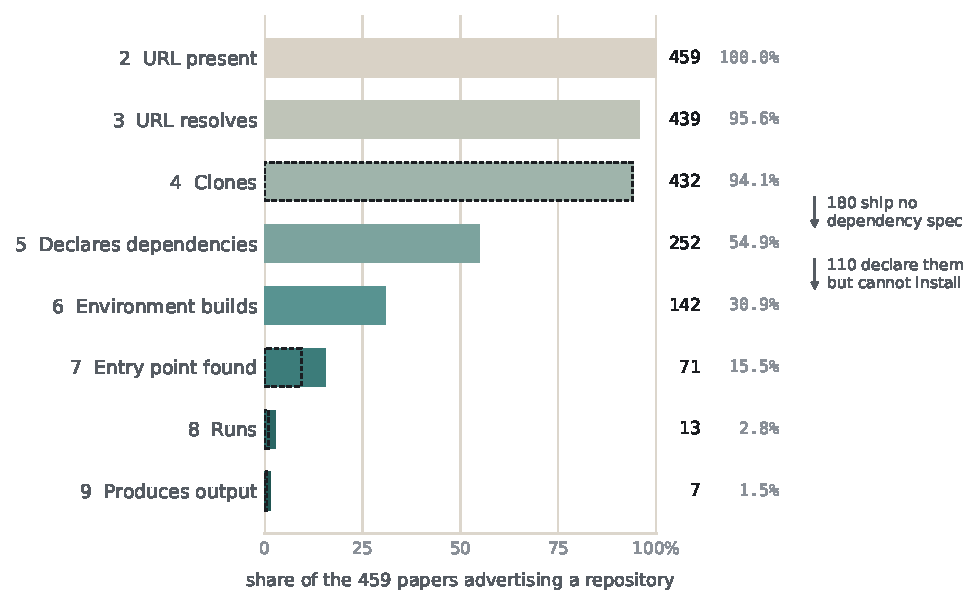
\includegraphics[width=\textwidth]{figures/attrition.pdf}
\caption{The attrition curve, $n=459$ arXiv quantitative-finance
machine-learning papers that advertise a code repository. Filled bars are the
primary specification; dashed outlines show the conservative entry-point rule
where it differs. The two large losses are annotated: they occur at declaring
and building an environment, not at link rot or at execution. Every value is
computed from the released records by \texttt{paper/make\_figures.py}.}
\label{fig:attrition}
\end{figure}

\begin{table}[H]
\centering
\caption{Attrition across the ladder, $n=459$ papers advertising a code URL.
The \emph{README} column is the primary specification, in which entry points may
be taken from the authors' own documentation; the \emph{convention} column
restricts entry points to conventionally named scripts. The two agree exactly
through rung 6, which are decided before any entry-point heuristic applies.}
\label{tab:attrition}
\small
\begin{tabular}{@{}clrrrr@{}}
\toprule
\# & Rung & \multicolumn{2}{c}{README (primary)} & \multicolumn{2}{c}{Convention only} \\
\cmidrule(lr){3-4}\cmidrule(lr){5-6}
   &      & $n$ & \% & $n$ & \% \\
\midrule
2  & \texttt{URL\_PRESENT}       & 459 & 100.0 & 459 & 100.0 \\
3  & \texttt{URL\_RESOLVES}      & 439 & 95.6  & 439 & 95.6 \\
4  & \texttt{CLONED}             & 432 & 94.1  & 431 & 93.9 \\
5  & \texttt{DEPS\_DECLARED}     & 252 & 54.9  & 252 & 54.9 \\
6  & \texttt{ENV\_BUILDS}        & 142 & 30.9  & 142 & 30.9 \\
7  & \texttt{ENTRYPOINT\_FOUND}  & 71  & 15.5  & 43  & 9.4 \\
8  & \texttt{RUNS}               & 13  & 2.8   & 5   & 1.1 \\
9  & \texttt{PRODUCES\_OUTPUT}   & 7   & 1.5   & 3   & 0.7 \\
\bottomrule
\end{tabular}
\end{table}

Three features of the curve carry the paper's content.

\emph{Link rot is real but modest.} Twenty of 459 advertised repositories
(4.4\%) no longer resolve, and one of those twenty is an extraction defect of
ours rather than a dead link, leaving nineteen (4.1\%) as measured rot. This is
the failure mode most often assumed to dominate, and it is the smallest of the
large drops. Two guards stand behind the figure. Because a transient resolver
failure is indistinguishable from a dead domain on a single attempt,
transport-level failures are retried before being recorded; without that, one
repository in this corpus would have been reported as rotted when it was live.
And because an address mangled by text extraction is likewise indistinguishable
from a dead one by status code, the normalization described above is asserted by
the audit script rather than assumed.

\emph{The first large drop is environment declaration.} Of the 432 repositories
that clone, 180 ship no dependency specification of any kind, taking the sample
from 94.1\% to 54.9\% in a single rung. Nothing exotic is required to clear it: a
\texttt{requirements.txt} suffices.

\emph{The second large drop is environment construction.} Of the 252
repositories that declare dependencies, 110 fail to install them, taking the
sample to 30.9\%. \Cref{tab:failure_mix} shows what the installer reported;
\Cref{tab:cohort} shows how the rate varies with the age of the paper. Neither
identifies a mechanism, for reasons given below.

\subsection{Why artifacts stop}\label{sec:failure_mix}

\Cref{fig:reasons} shows every reason an artifact stopped, grouped by the rung
that blocked it; \Cref{tab:failure_mix} gives the same counts as a table. The
single largest bar is not a technical failure at all: 180 repositories ship no
dependency specification, so there is nothing to install.

\begin{figure}[H]
\centering
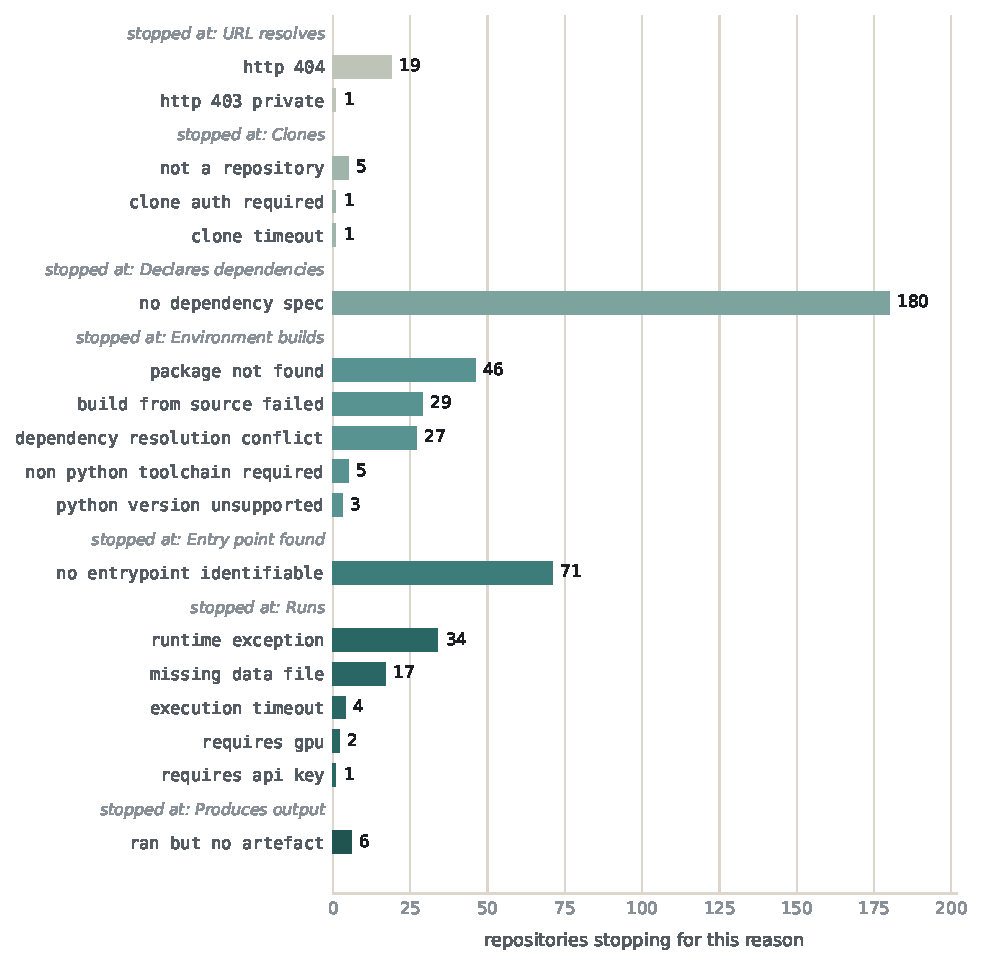
\includegraphics[width=0.92\textwidth]{figures/reasons.pdf}
\caption{Why artifacts stop, primary specification. Each bar counts the
repositories that stopped at the named rung for the named reason; the 452 bars
sum, with the seven artifacts that cleared every mechanical rung, to the full
sample of 459.}
\label{fig:reasons}
\end{figure}

\begin{table}[H]
\centering
\caption{Failure mix by blocking rung, primary specification. Counts are
repositories stopping at that rung for that reason.}
\label{tab:failure_mix}
\small
\begin{tabular}{@{}llr@{}}
\toprule
Rung & Reason & $n$ \\
\midrule
\texttt{URL\_RESOLVES}     & \texttt{http\_404}                       & 19 \\
                           & \texttt{http\_403\_private}              & 1 \\
\midrule
\texttt{CLONED}            & \texttt{not\_a\_repository}              & 5 \\
                           & \texttt{clone\_timeout}                  & 1 \\
                           & \texttt{clone\_auth\_required}           & 1 \\
\midrule
\texttt{DEPS\_DECLARED}    & \texttt{no\_dependency\_spec}            & 180 \\
\midrule
\texttt{ENV\_BUILDS}       & \texttt{package\_not\_found}             & 46 \\
                           & \texttt{dependency\_resolution\_conflict}& 27 \\
                           & \texttt{build\_from\_source\_failed}     & 29 \\
                           & \texttt{non\_python\_toolchain\_required}& 5 \\
                           & \texttt{python\_version\_unsupported}    & 3 \\
\midrule
\texttt{ENTRYPOINT\_FOUND} & \texttt{no\_entrypoint\_identifiable}    & 71 \\
\midrule
\texttt{RUNS}              & \texttt{runtime\_exception}              & 34 \\
                           & \texttt{missing\_data\_file}             & 17 \\
                           & \texttt{execution\_timeout}              & 4 \\
                           & \texttt{requires\_gpu}                   & 2 \\
                           & \texttt{requires\_api\_key}              & 1 \\
\midrule
\texttt{PRODUCES\_OUTPUT}  & \texttt{ran\_but\_no\_artefact}          & 6 \\
\bottomrule
\end{tabular}
\end{table}

The environment failures divide into three roughly comparable mechanisms.
\texttt{package\_not\_found} (46) is a pinned dependency that has left the index;
\texttt{build\_\allowbreak from\_\allowbreak source\_\allowbreak failed} (29) is a
package with no current wheel that fails to compile;
\texttt{dependency\_\allowbreak resolution\_\allowbreak conflict} (27) is the
residual, and it is a weaker label than its name suggests. It is the classifier's
fallthrough, so it collects genuine pin conflicts together with build-backend
errors that resist finer classification. We report it as a bucket rather than a
mechanism, and a reader wanting the split can recover it from the stored
installer output in the released records. All three are properties of elapsed
time rather than of the authors' diligence at submission. Whether that amounts to
decay is a question the corpus can be asked directly, and the answer is more
qualified than we first assumed.

\begin{table}[H]
\centering
\caption{Environment construction by publication cohort, primary specification.
Cohort is the year in the arXiv identifier's \texttt{YYMM} prefix, that is the
month the paper was announced and the artifact became publicly reachable, which
is the clock an aging artifact runs on. Three of the 459 records were submitted
in the calendar year before their identifier was issued and would fall one
cohort earlier under the corpus \texttt{year} field; two of those sit on the
2025/2026 boundary and move 137/68 to 139/66. The rightmost column, and every
claim drawn from it, is identical under either rule. That column conditions on
the repository having declared dependencies at all, so it isolates whether a
declared environment can still be built.}
\label{tab:cohort}
\small
\begin{tabular}{@{}lrrrr@{}}
\toprule
Cohort & $n$ & Declares deps & Builds & Builds $\mid$ declares \\
\midrule
2015--2022 & 64  & 45.3\% & 18.8\% & 41.4\% \\
2023       & 68  & 54.4\% & 22.1\% & 40.5\% \\
2024       & 122 & 49.2\% & 27.0\% & 55.0\% \\
2025       & 137 & 61.3\% & 38.7\% & 63.1\% \\
2026       & 68  & 61.8\% & 42.6\% & 69.0\% \\
\bottomrule
\end{tabular}
\end{table}

The gradient is real but modest, and it is not monotone: conditional on declaring
dependencies, a 2026 artifact builds about 1.7 times as often as one from 2022 or
earlier, and the 2023 cohort sits marginally below the oldest one. An earlier
version of this table showed a threefold gradient; roughly half of it was a
defect in our own container image, which penalized exactly the older repositories
most likely to need a source build (\Cref{sec:harness_defects}). We report the
corrected figures and note that our first, more striking result was wrong in the
direction we would have liked.

Two readings fit what remains, and a single cross-section cannot separate them.
Artifacts may decay as they age, or practice may simply be improving, so that
recent authors write more buildable environments than their predecessors did.
Both are plausible, and at this effect size neither is strongly supported.

The reason mix argues against attributing the gradient wholly to the mechanism we
had assumed. If aging worked mainly through packages leaving the index, then
\texttt{package\_not\_found} should claim a growing share of older cohorts. It
does not: as a fraction of repositories that declare dependencies it is 17.2\%
for 2015--2022, 29.7\% for 2023, 16.7\% for 2024, 16.7\% for 2025 and 14.3\% for
2026, which is flat within sampling noise. The honest statement is that older
artifacts build less often, that the mechanism is not identified by these data,
and that separating decay from cohort requires re-scoring this corpus later
rather than reasoning across it now. The harness is released so that measurement
can be made.

This also means the measurement is timestamped: the same corpus scored two years
hence is unlikely to score the same, and any comparison against these figures
must carry their date.

At the execution rung, the seventeen \texttt{missing\_data\_file} outcomes are
substantive, though the label is broader than its name. The classifier routes any
report of an absent path to this bucket, which covers two situations: a
repository that fetches its inputs at run time and is blocked because network
access is denied during execution by design, and a repository whose expected
input file simply is not in the distribution. Both mean the same thing for a
reader, which is why they share a rung, and neither is rescued by our
connectivity: the artifact as released does not carry what it needs. They are not
separated in the counts, and a reader wanting the split can recover it from the
per-record detail in the released data, which is now retained at full length for
this purpose.

\subsection{Defects found in our own instrument}\label{sec:harness_defects}

A study that measures how often other people's code silently fails is obliged to
report how often its own did. Four defects were found after a first campaign had
completed, and they did not all err in the same direction. Three inflated the
failure rate, in the direction this study's hypothesis predicted, which is why
they were hard to see: a harness that agrees with you invites less scrutiny. The
fourth did the opposite and manufactured a success, which is the error a reader
should worry about more, and it was caught only because the output was read
rather than counted.

\emph{The container image lacked a toolchain.} The base image was
\texttt{python:3.11-slim}, which ships neither \texttt{git} nor a C compiler. A
repository whose requirements name a \texttt{git+https} dependency, or whose
wheel must be compiled, therefore failed to install for a reason belonging to our
image. Seven repositories were affected, four for want of \texttt{git} and three
for want of a compiler.

\emph{The clone was shallow.} \texttt{git clone -{}-depth 1} fetches no tags, and a
package whose version is derived by \texttt{setuptools-scm} then fails with
``unable to detect version''. Eight repositories failed to build for that reason
alone. A reader following the paper's URL clones normally and sees none of this.

\emph{A bare \texttt{make} was accepted as an entry point.} The documented rule
has always been that a command taken from a README must name a target that
exists; the code checked only that a \texttt{Makefile} was present. One
repository's default target printed the Makefile's own usage message, and an
interim run recorded that as the artifact producing output at rung 9. This is the
defect that ran the wrong way: it created a success rather than a failure, and it
would have added an eighth paper to the headline count. It is the second such
case in this project's history, the first being a vendored tokenization library
whose bundled demo satisfied the naming heuristic for two papers
(\Cref{sec:ladder}); both are visible in the superseded result files released
alongside the current ones.

\emph{URL normalization stripped only trailing characters}, as described in
\Cref{sec:corpus}.

The first three matter for the shape of the curve, not merely its level. Older
repositories are the ones most likely to need a source build or a \texttt{git}
dependency, so the missing toolchain penalized them disproportionately.
Conditional on declaring dependencies, the 2015--2022 cohort builds 41.4\% of the
time under the corrected harness and 20.7\% under the defective one, while the
2026 cohort is unchanged at 69.0\%. Roughly half of what had looked like an age
gradient was our own image. The remaining gradient is reported in
\Cref{tab:cohort} and is considerably milder.

We report this at length because the alternative was to report a cleaner result
that we knew to be partly an artifact, and because the pattern is the paper's own
argument turned on itself: the defects were invisible precisely because their
output was plausible.

\subsection{Not every advertised repository is the paper's own}\label{sec:shared_repos}

The 459 records point to 427 distinct repositories. Twenty-five addresses are
advertised by more than one paper, accounting for 57 records, and inspection of
that list shows what is happening: several are widely used third-party libraries
rather than a paper's released code. A paper that names the data client or the
modeling toolkit it used, in the same sentence pattern a paper uses to announce
its own repository, is indistinguishable to an extractor working from prose.

These records behave differently enough to matter. Repositories shared between
papers clone 100.0\% of the time against 93.3\% for the rest, declare
dependencies 86.0\% against 50.5\%, and build 50.9\% against 28.1\%. That is what
a maintained library looks like. But they yield an entry point 14.0\% of the time
against 15.7\%, and \emph{none} of them produces output, because a library has no
analysis to run. Including them therefore lifts the middle of the curve
while contributing nothing at the top, which flatters the environment rungs and
makes the drop from rung 6 to rung 9 look steeper than it is for the papers'
own artifacts.

We report the unscreened curve as primary because the screening rule we can
implement is a heuristic in its own right, and substituting one heuristic for
another silently would be worse than disclosing this one. A reader who wants the
screened figure can recompute it from the released records, and the direction of
the bias is stated here so that no one has to guess at it. The effect on the
paper's conclusion is small and adverse to our own headline: excluding shared
repositories would lower the environment rungs and leave the seven rung-9
artifacts untouched.

\subsection{Sensitivity to the entry-point heuristic}\label{sec:sensitivity}

Identifying what to run is the most discretionary step, so the study is run in two
configurations. Restricting to conventionally named scripts finds an entry point
in 43 repositories; additionally accepting a command documented in the
repository's own README finds 71. The looser specification raises the number that
execute from 5 to 13 and the number that emit output from 3 to 7.

The sensitivity carries through to the top of the ladder, and it must be reported
there because that is where it bites hardest. The single artifact scored
\emph{match} at rung 10 is reached only by the README route: under the
conservative rule it never clears rung 7. Of the three artifacts that do emit
output under that rule, two are the bundled self-tests of
\Cref{sec:rung10_results}. The third is the timing case described above: a
completed portfolio backtest, which is a more substantial run than anything in
the primary rung-9 set apart from the match itself. It was adjudicated
separately and scored \emph{not comparable}, on two grounds: the paper's abstract
states no recoverable numeric claim, reporting only that the method
``significantly outperforms'' its baselines, and the run seeds itself randomly
and says so in its own output, so a second run would emit different values. The
adjudicated match count is therefore one under the primary specification and zero
under the conservative one, with all eight adjudications released in the
worksheet. The adjudicated match count is therefore one under the
primary specification and zero under the conservative one. Stopping the sensitivity analysis at rung 9, where the two columns still
show a difference of degree, would have concealed the one place where the
headline changes in kind.

The two configurations agree on rungs 2 through 6 for 458 of the 459
repositories, and the audit script checks that they agree to within that
tolerance. Both exceptions we have observed are wall-clock effects rather than
scoring disagreements, and both are worth stating because they bound how
reproducible these figures are.

One repository cloned in one run and hit the ten-minute clone timeout in the
other. Unlike the resolution check at rung 3, the clone is not retried, so a slow
transfer is recorded as a failure. A second repository, with the same
conventionally named entry point selected in both runs, completed in 1{,}667
seconds under one configuration and exceeded the 1{,}800-second execution budget
under the other. It is therefore the one record whose conservative rung
\emph{exceeds} its primary rung, so the conservative set is not a subset of the
primary at rungs 8 and 9 even though the entry-point rule is strictly stricter.
Three artifacts emit output under the conservative rule and seven under the
primary, but the two sets are not nested: one member of the smaller set is absent
from the larger.

The practical reading is that the mechanical rungs are reproducible to within
about one repository, that the upper rungs additionally carry timing sensitivity
for artifacts whose runtime sits near the budget, and that a headline of seven is
seven plus or minus one rather than an exact count.

The gap between the columns is the honest measure of how much of the upper curve
is our conservatism rather than the literature's. It is large in relative terms
and small in absolute terms: on either specification, fewer than one paper in
thirty executes to completion unassisted, and fewer than one in sixty emits
output.

\subsection{Comparison with the earlier, smaller campaign}\label{sec:replication}

An earlier campaign scored a 154-paper sample. Those 154 papers are a strict
subset of the present 459: the corpus was extended rather than redrawn, so every
paper in the earlier campaign is also in this one. We state that plainly because
comparing the subset against the superset that contains it would not be a
replication, and reporting it as one would be the most misleading thing in this
paper.

Nor can the two campaigns be compared as repeated measurements. The harness
changed between them, and not cosmetically: the container image gained a
toolchain, the clone stopped being shallow, and the entry-point rule was
tightened (\Cref{sec:harness_defects}). Five of the 154 records differ across the
campaigns at rungs 2 to 6, and all five are consequences of those revisions. The
comparison therefore measures our corrections, not the literature, and we draw no
stability conclusion from it.

What can be compared out of sample is the 305 papers that entered with the
expansion and that the earlier campaign never saw, scored under the same harness
as everything else. Restricting to rungs 2 through 6, the earlier 154 score
resolution 94.2\%, cloning 89.6\%, dependency declaration 53.9\% and environment
construction 27.9\%; the 305 added papers score 96.4\%, 96.4\%, 55.4\% and
32.5\%. Declaration differs by 1.5 percentage points and construction by 4.5.

Those crude gaps should not be read as stability, and the reason is worth setting
out because it is easy to miss. The two partitions have very different age
profiles: the earlier 154 contain no paper announced before 2024, while the added
305 reach back to 2015 and are 21\% pre-2023. Within every cohort the two
partitions share, the added papers build far more often than the earlier ones:
29.0\% against 13.3\% for 2024, 62.5\% against 25.8\% for 2025, and 61.1\%
against 36.0\% for 2026. Standardizing the added partition's cohort-specific
rates onto the earlier partition's age mix gives 58.8\% against 27.9\%, a gap of
thirty points rather than four and a half.

The near-agreement in the crude figures is therefore composition canceling
outcome: the added sample is older, which lowers its overall rate, and better
within each cohort, which raises it. We do not know why the two partitions differ
so much within cohort. It is not the seed set carried over from earlier work
(excluding it leaves the earlier partition at 28.4\%), and it is not where the
URL was found (papers whose URL came from the abstract and from the full text
build 26.5\% and 32.1\% of the time respectively, a gap far smaller than the one
to be explained). The honest reading is that the two draws
are not exchangeable, that we cannot say what distinguishes them, and that this
study therefore has no strong out-of-sample check. The shape of the curve, two
large losses at declaration and construction, is common to both partitions; the
levels are not.

\subsection{Rung 10}\label{sec:rung10_results}

Seven repositories produced output and are therefore eligible for the final rung,
which asks whether an emitted number matches a headline number in the paper. All
seven were adjudicated by hand against the paper's own numeric claims; the
worksheet pairing each artifact's captured stdout with those claims is released
with the corpus so the judgments can be inspected and disputed. One was scored
\emph{match} and six \emph{not comparable}. We give the count rather than a rate:
seven cannot support a percentage.

Reading the seven is more informative than counting them, because it shows that
rung 9 is a weaker rung than its name suggests. Emitting output is not the same
as running the analysis. Two artifacts executed a bundled self-test that reports
tensor shapes and losses on synthetic inputs. One ran a correctness validator
that skipped every GPU check because the CUDA extensions were not built, which
is precisely where the paper's throughput claims come from. One completed a
walk-forward experiment whose data fetch returned nothing for every ticker, so
the analysis ran on an empty universe. One terminated on a missing API key, and
the captured output is that error. One ran a data-acquisition step that wrote
files and printed nothing.

The single \emph{match} is instructive about what success looks like, and it was
checked against the published table rather than taken on the script's word. The
repository documents \texttt{finalscripts/table1.py}; running it regenerates the
paper's Table 1 in full, on the same 14-variable panel, and every one of the
thirty-six reported values agrees exactly: recall, precision, $F_1$ and mean
signed offset for all nine methods, from \texttt{LLM only} at
$0.77/0.87/0.82/{+}3.1$ through the four data-only baselines to the four
cross-validated variants, ending at $0.88/0.77/0.82/{+}0.9$. The best $F_1$ of
0.82 is the figure the abstract headlines. Presentation differs without
disagreeing: the manuscript labels the combined rows differently from the script,
reports an $F_2$ column the script omits, and omits the raw hit and false-alarm
counts the script prints.

What reproduced, however, is narrower than ``regenerates Table 1'' suggests, and
the artifact says so itself. Its output header reports \texttt{new API calls =
0}: the language-model stage over central-bank minutes, which is the paper's
distinctive contribution, is replayed from model outputs committed to the
repository rather than recomputed. Network access is denied during execution, so
it could not have been otherwise. What runs end to end is the statistical
validation and scoring on stored text-derived candidates, which is a real and
unusually well-packaged result, but it is not the text pipeline. We record this
because a paper arguing that ``reproduced'' is used too loosely cannot afford to
use it loosely about its own single success.

One artifact in 459 regenerated a published table on a clean machine, from the
URL the paper gives its readers, without network access and without contacting
anyone, on model outputs the authors had the foresight to commit.

That the sample thins from 459 to seven, and from seven to one, is itself the
finding: the question the rung was designed to answer is, for this corpus, very
nearly unanswerable, because almost nothing gets far enough to ask it of.

\section{Discussion}\label{sec:discussion}

\subsection{Reading this against the coordinated-study result}\label{sec:vs_perignon}

The natural comparison is \citet{Perignon2024}, who report 52\% exact
reproduction in finance. Nothing here contradicts that number; the two measure
different situations, and the distance between them is the useful quantity.

In the coordinated setting, code is written by a participating team knowing it
will be run, the raw data are supplied, and the researchers are reachable. In
ours, the artifact is whatever a published paper points its readers to, retrieved
cold, on a clean machine, with no data supplied and nobody to ask. The first
measures whether finance code \emph{can} reproduce. The second measures whether a
reader can get it to run at all.

That the figures are 52\% and 2.8\% does not mean the coordinated result was
optimistic. It means most of what that measurement captures is supplied by
conditions surrounding the code rather than by the artifact itself: the data, the
authors' attention, the knowledge that someone will check. Strip those away and
what remains is the artifact as released, which is what a reader inherits. The
practical implication in \Cref{sec:where} follows directly: the interventions
that would move our number are the ones that make an artifact self-contained,
not the ones that make an author more careful at submission.

\subsection{What the curve licenses us to say}\label{sec:claim_scope}

The measured quantity is narrow and worth stating precisely. Of 459
quantitative-finance machine-learning papers that advertise a code repository,
thirteen executed to completion and seven produced output when a stranger cloned
the repository, built the declared environment in a container, and ran the
documented entry point without correspondence, manual repair, or reading beyond
the README.

That is not a claim that the other 452 papers are wrong, and it is not a
replication failure rate. It is a statement about artifacts, not findings: the
released code, as released, does not run unassisted on a current platform.
Several of the failures are ones an author could resolve in a message and a
motivated reader in an afternoon. The claim is about the cost of that
afternoon, multiplied across a literature.

The converse also holds, and the seven adjudicated artifacts make it concrete.
Producing output says nothing about whether the output is the paper's: two ran a
bundled self-test on synthetic inputs, one skipped every GPU measurement the
paper's claims depend on, one analyzed an empty universe after its data fetch
returned nothing, and one printed an authentication error. Clearing rung 9
establishes that a program ran, not that the study did.

\subsection{Where the attrition actually happens}\label{sec:where}

The practical value of an ordered ladder is that it localizes the loss, and the
location is not where the reproducibility discourse usually points. Link rot,
the most-discussed failure, accounts for 4.4\%. The two large drops are
environment declaration (180 repositories ship no dependency specification) and
environment construction (110 of the 252 that declare one no longer install).

These have different remedies. The first is a submission-time omission and is
cheap to fix: a \texttt{requirements.txt} clears it, and an editorial checkbox
would move the number.

The second is harder to prescribe for, because we cannot identify its mechanism.
A declared environment can fail to build because a pinned package has left the
index, because a pin set no longer admits a solution, or because a source
distribution no longer compiles, and the three are of comparable size. It is
tempting to read all of them as aging, and \Cref{tab:cohort} does show older
cohorts building far less often. But \Cref{sec:limitations} sets out why that
reading is not established: a cross-section cannot separate aging from a change
in practice, and \texttt{package\_not\_found} does not grow as a share of older
cohorts, which is what a pure index-attrition story predicts.

What can be said is weaker and still useful for policy. A journal that requires a
dependency file addresses the larger drop immediately, and that recommendation
does not depend on any mechanism. A journal that wants artifacts to survive five
years needs artifacts that pin more than package versions, in practice a
container image or a lockfile with hashes, and should know that this is a bet
against several failure modes at once rather than a fix for one identified
cause.

\subsection{Limitations}\label{sec:limitations}

\emph{The entry-point heuristic is the binding constraint on the upper rungs.}
Between rungs 6 and 8 the measurement is partly measuring us. We report both
specifications (\Cref{sec:sensitivity}) rather than choosing one, but neither
matches a determined human who would read the source, infer the intended
invocation, and supply arguments. The upper rungs are therefore a lower bound on
what a persistent reader could achieve.

\emph{The corpus is arXiv and recent.} Fields whose authors do not preprint are
absent, and the sample is weighted toward the last two years. The curve describes
current arXiv practice in quantitative finance.

\emph{The measurement is timestamped, and the direction is not established.}
Older cohorts build markedly less often (\Cref{tab:cohort}), but a single
cross-section cannot separate artifacts decaying with age from practice improving
over time, and the reason mix does not support attributing the gradient to
packages leaving the index: \texttt{package\_not\_found} is flat as a share of
dependency-declaring repositories across cohorts. What follows is only that any
comparison against these figures must be dated, and that establishing a decay
rate requires re-scoring this corpus later rather than reading aging off a
cross-section. That is part of why the harness is released rather than only the
numbers.

\emph{Time and resource budgets bind.} Dependency installation is capped at
fifteen minutes per artifact and execution at thirty, on two allocated cores and
eight gigabytes of memory
without a GPU. Four repositories hit that ceiling
and are recorded as timeouts, not failures of a different kind. An artifact whose
honest runtime is a day on a cluster is not distinguishable here from one that
hangs.

\emph{Rung 10 is human-scored, and specification-dependent.} The final rung
reflects one scorer's judgment about whether an emitted number corresponds to a
published claim. With seven eligible artifacts this is disclosed as adjudication
rather than measurement, and the worksheet, including the reasoning for every
verdict, is released so that the judgments can be checked. The count is also not
robust to the entry-point rule: the single match is reached only under the
README specification, and is zero under the conservative one
(\Cref{sec:sensitivity}). A count of one that becomes zero under a defensible
alternative should be read as a bound, not a rate. The \emph{match} was verified against the published
table cell by cell, all thirty-six values; the six \emph{not comparable} verdicts
turn on what the artifact executed rather than on any numerical tolerance, which
makes them easier to dispute and easier to check.

\subsection{The harness as the durable contribution}\label{sec:harness_contribution}

The numbers in \Cref{sec:results} describe one corpus at one moment. The
instrument that produced them is the part intended to outlast the snapshot: it is
installable, it takes any corpus of paper identifiers and code URLs, and it emits
per-artifact records with a closed failure vocabulary.

Three properties were built in because their absence would have been invisible in
the output. Harness-attributable failures carry a distinct reason code and are
excluded from claims about the literature. Conditions indicating harness
misconfiguration raise an error rather than being recorded as data, so a broken
run fails loudly instead of producing a clean-looking corpus of false negatives.
And the discretionary heuristic is a switch rather than a constant, so its effect
is reportable instead of assumed.

Those choices were not precautionary in the abstract. During development, a
container backend that installed dependencies in one container and executed in
another produced a complete, plausible, entirely false result in which nothing in
the corpus ran; it was caught because the failures took a tenth of a second. A
study that measures how often other people's code silently fails to work is
poorly placed to assume its own does.

\subsection{Future work}\label{sec:future}

Three extensions are supported by the released artifact. The corpus can be widened
beyond arXiv and beyond finance, since nothing in the ladder is domain-specific.
The same corpus can be re-scored periodically to measure the decay rate directly,
converting a limitation into a result. And the entry-point step can be
strengthened, ideally by comparing the automated heuristics against a
human-annotated subset, which would replace the sensitivity band with a
calibration.


\bibliographystyle{apalike}
\bibliography{bib/references}

\end{document}
